This section describes the schema currently used to store \glspl{fragility model}, which are required for the Scenario Damage Calculator. A \gls{fragility model} can be comprised of several \glspl{fragility function}, describing the probability of exceeding a set of limit, or damage, states. These \glspl{fragility function} can be defined in two ways: discrete or continuous. In the former manner, sets of probabilities of exceedance (one set per limit state) are defined for a list of intensity measure levels, as illustrated in Figure~\ref{fig:fragModelDiscrete}.

\begin{figure}[ht]
\centering
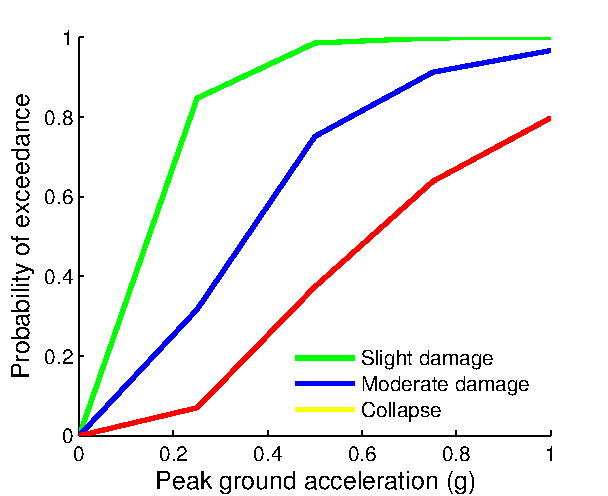
\includegraphics[width=8cm,height=6cm]{figures/risk/DisFragilityModel.pdf}
\caption{Graphical representation of a discrete fragility model.}
\label{fig:fragModelDiscrete}
\end{figure}

Similarly to what has been described for the \glspl{vulnerability model}, the NRML schema for this input also has some attributes that are common to all of the \glspl{fragility function} comprising the model. This initial portion of the schema is depicted below:

\begin{Verbatim}[frame=single, commandchars=\\\{\}, samepage=true]
<?xml version="1.0" encoding="UTF-8"?>
<nrml xmlns:gml="http://www.opengis.net/gml"
      xmlns="http://openquake.org/xmlns/nrml/0.4">
<\textcolor{red}{<fragilityModel format="discrete">}>
    <\textcolor{green}{description} "Fragility Model for RC" <\textcolor{green}{/description}>
    <\textcolor{green}{limitStates}
        slight
        moderate
        collapse
    <\textcolor{green}{/limitStates}>
    ...
\end{Verbatim}

\begin{itemize}
\item  \Verb+description+: represents an attribute that can be used to include  some information about the \gls{fragility model}, for example, what building typologies are being covered or the source of the \gls{fragility model};
\item  \Verb+limitStates+: this field is used to define the number and nomenclature of each limit state. Despite the fact that three limit states are being employed in this example, it is possible to use any number of states, as long as a fragility curve is always defined for each limit state.
\end{itemize}

\begin{Verbatim}[frame=single, commandchars=\\\{\}, samepage=true]
    ...
    <\textcolor{green}{ffs noDamageLimit= 0.05}>
        <\textcolor{blue}{taxonomy} RC <\textcolor{blue}{/taxonomy}>
        <\textcolor{blue}{IML} IMT="PGA" imlUnit="g"> 0.0 0.25 0.50 0.75 1.00 <\textcolor{blue}{/IML}>

        <\textcolor{blue}{ffd} ls="slight">
            <\textcolor{magenta}{poes}> 0.0 0.85 0.98 0.99 1.00 < \textcolor{magenta}{/poes}>
        <\textcolor{blue}{/ffd}
        <\textcolor{blue}{ffd} ls="moderate">
            <\textcolor{magenta}{poes}> 0.0 0.32 0.75 0.91 0.97 < \textcolor{magenta}{/poes}>
        <\textcolor{blue}{/ffd}
        <\textcolor{blue}{ffd} ls="collapse">
            <\textcolor{magenta}{poes}> 0.0 0.07 0.37 0.64 0.80 < \textcolor{magenta}{/poes}>
        <\textcolor{blue}{/ffd}
    <\textcolor{green}{/ffs}>
<\textcolor{red}{/fragilityModel}>
</nrml>
\end{Verbatim}

For each building typology, a set of limit state curves need to be stored within the field \Verb+ffs+ (fragility function set). The following attributes are currently being employed to define this input:

\begin{itemize}
\item  \Verb+noDamageLimit+: this attribute defines the intensity measure level below which the probability of exceedance for all curves is zero;
\item  \Verb+taxonomy+: a unique key that is used to relate each \gls{fragility function} with the relevant \glspl{asset} in the \gls{exposure model};
\item  \Verb+IML+: this attribute serves the purposes of defining the list of intensity measure levels for which the limit state curves are defined. In addition, it is also necessary to define the intensity measure type (\Verb+IMT+) being used and the respective units (\Verb+imlUnit+);
\item  \Verb+ffd+: this field (fragility function discrete) is used to define the probabilities of exceedance (\Verb+poes+) of each limit state curve. It is also necessary to include which limit state is being defined in the attribute \Verb+ls+.
\end{itemize}

As previously mentioned, the user may choose to define the \glspl{fragility function} in a continuous manner, through the use of cumulative lognormal functions. In Figure~\ref{fig:fragModelContinuous}, a continuous fragility model is presented.

\begin{figure}[ht]
\centering
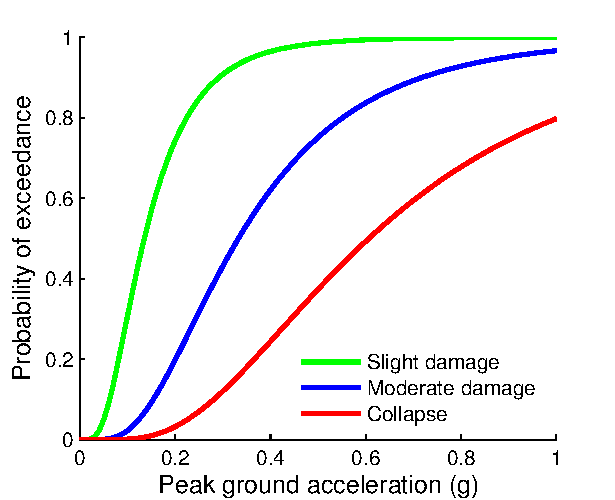
\includegraphics[width=8cm,height=6cm]{figures/risk/ConFragilityModel.pdf}
\caption{Graphical representation of a continuous fragility model.}
\label{fig:fragModelContinuous}
\end{figure}

The NRML schema to store these functions has an initial structure similar to that described for the discrete \glspl{fragility model}. Then, the continuous limit state curves are stored as illustrated below:

\begin{Verbatim}[frame=single, commandchars=\\\{\}, samepage=true]
    ...
    <\textcolor{green}{ffs noDamageLimit= 0.05}>
        <\textcolor{blue}{taxonomy} RC <\textcolor{blue}{/taxonomy}>
        <\textcolor{blue}{IML} IMT="PGA" minIML="0.0" maxIML="1.0" imlUnit="g" ><\textcolor{blue}{/IML}>
        <\textcolor{blue}{ffd} ls="slight">
            <params \textcolor{magenta}{mean}="0.16" \textcolor{magenta}{stddev}="0.11" />
        <\textcolor{blue}{/ffd}
        <\textcolor{blue}{ffd} ls="moderate">
            <params \textcolor{magenta}{mean}="0.40" \textcolor{magenta}{stddev}="0.26" />
        <\textcolor{blue}{/ffd}
        <\textcolor{blue}{ffd} ls="collapse">
            <params \textcolor{magenta}{mean}="0.73" \textcolor{magenta}{stddev}="0.48" />
        <\textcolor{blue}{/ffd}
    <\textcolor{green}{/ffs}>
<\textcolor{red}{/fragilityModel}>
</nrml>
\end{Verbatim}

Again, the set of limit state curves for each building typology needs to be stored within the field \Verb+ffs+ (fragility function set), through the definition of the following attributes:

\begin{itemize}
\item  \Verb+noDamageLimit+: this attribute defines the intensity measure level below which the probability of exceedance for all curves is zero;
\item  \Verb+type+: this parameter defines the type of probabilistic distribution being used to define the limit state curves. Currently the engine only supports lognormal distributions, however, the capability of considering other types of distributions (e.g. normal, exponential) will be developed in the future;
\item  \Verb+taxonomy+: a unique key that is used to relate each \gls{fragility function} with the relevant \glspl{asset} in the \gls{exposure model};
\item  \Verb+IML+: in this field, the intensity measure type (\Verb+IMT+) and associated units (\Verb+imlUnit+) for the limit state curves is defined, along with the minimum (\Verb+minIML+) and maximum (\Verb+maxIML+) intensity measure levels enclosing the range of applicability of the set of fragility functions;
\item  \Verb+ffc+: this field (fragility function continuous) is used to define the mean (\Verb+mean+) and standard deviation (\Verb+stddev+) of the cumulative lognormal function. In addition, the limit state for the curve being defined needs to be specified in the attribute \Verb+ls+.
\end{itemize}